\chapter{Overview of the Logistics of HYPERION}
\label{chap:logistics}

We must now find a way to test our hypotheses about building a 
monopole-sensitive interferometer. Ideally we would do this in multiple steps, 
graduating from tests that use the fewest resources up to the most expensive 
tests, and would conclude with a full deployment of the array with which to 
observationally test our ideas and attempt to make a measurement of the 
monopole reionization signal. 

This leads us to a natural starting point: to build a simulation of our array.  
This can be done cheaply and relatively quickly, and can give us a sense of 
whether or not this idea has any potential merit.

\section{Methodology of Simulation}

Fundamentally, we will be doing all the same steps that have been laid out in 
the previous three chapters. We will create a model sky and a model array, and 
then calculate the visibilities for each baseline separation of that array. We 
will then examine these visibilities to see if we have any sensitivity to the 
monopole term at all, and if so what form they take.

For our simulation, we first import a model array, which enables us to carry 
around a known geometry and baseline separations, along with individual antenna 
beam patterns and accessible frequencies. With this information and the 
previously made sky maps, we are now able to calculate our visibilities across 
many frequencies by using Eq.~\eqref{eq:vis}.

More importantly, the antenna beam information within the model array is itself 
a convenient way to import absorbers into the simulation.  Essentially, within 
the context of the simulation, the absorbers act as a modification term on the 
beam pattern, changing the way that each individual antenna sees the sky.

\subsection{Antenna Design and Primary Beam}

To start, we need a beam. HYPERION uses SARAS-style fat dipole antennas in our 
instrument, which means we will be using a frequency-invariant dipole beam 
pattern in our simulation to match~\citep{patra2013}.  This is the base beam 
model used throughout the simulation, calculated using 
Eq.~\eqref{eq:dipole-beam}.

\begin{equation}
    \label{eq:dipole-beam}
    A(\theta, \phi, \nu) = \cos\Big(\frac{\frac{\pi}{2} 
    \cos{\theta}}{\sin{\theta}}\Big)
\end{equation}

This frequency-invariance is important, as it removes one dangerous source of 
calibration errors in the experiment. Were there to be a changing beam shape 
due to frequency, then the improper calibration of those changes could 
introduce false signatures into the data.

\subsection{Absorber Baffles}

Now that we have a baseline antenna beam, we can begin the modification 
process. The effective antenna beam be calculated using 
equations~\eqref{eq:absorber-baffle} and~\eqref{eq:absorber-beam}.

In the construction of the absorber baffles within the simulation, the 
parameters we can play with are the absorptivity of the material (i.e.  how 
much attenuation does the absorber provide at each frequency), the height of 
the absorber walls, and how smooth the transition from absorber to sky is.  

So the first question is: how absorptive is our absorber at each frequency? To 
date, we are still relatively early in the testing of our hypothesis that 
absorber walls or ``baffles" between antennas will enable us to better observe 
the spatial monopole with an interferometer.  There have been two main sets of 
tests performed so far -- one in-lab test to measure the absorptivity of 
various proposed materials, and some brief field tests to gauge the 
effectiveness of our absorber at mitigating cross-talk between antennas.

The in-lab test was, in essence, a simple antenna return-loss measurement. To 
conduct the measurements, we started by constructing a large (i.e. 4.5' cube) 
Faraday cage out of wood and chicken wire, and placed an antenna at its center.  
From this setup, we could perform a simple return loss measurement and see what 
the maximum power return to the antenna is.

We could then line the cage with various absorptive materials and take another 
return-loss measurement, this time with (ideally) much of the power absorbed by 
the absorber, and see how effective each material is at dissipating energy 
within our science band. One such measurement is shown in 
Fig.~\ref{fig:fe-absorption}, featuring our most promising absorber candidate 
material, ferrite tiles.

\begin{figure}
    \begin{center}
    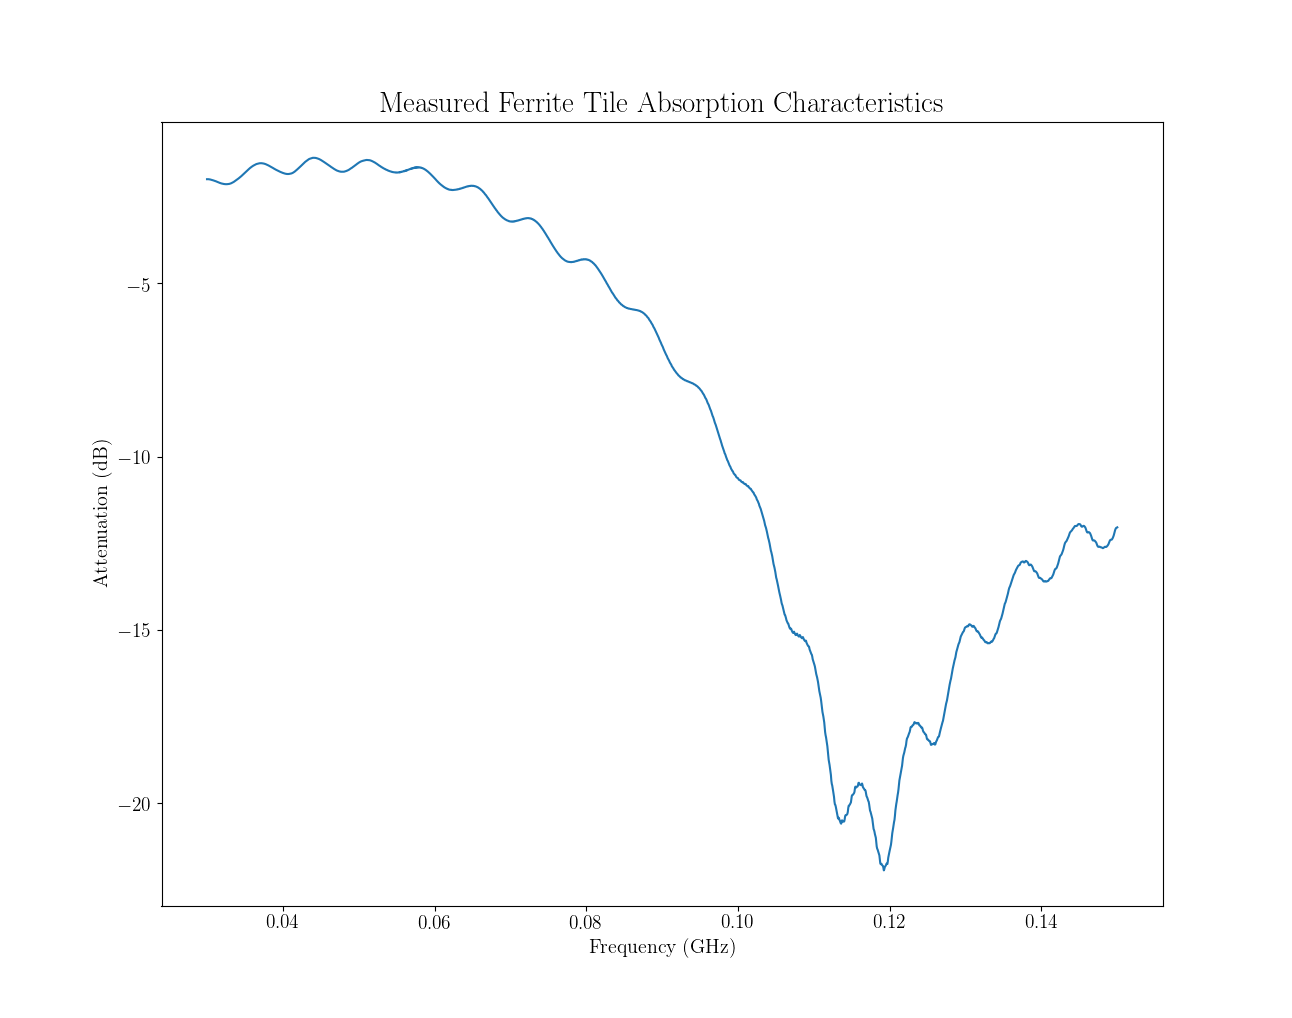
\includegraphics[width=\linewidth]{fe_absorption.png}
    \end{center}
    \caption{
        Here we see the results of a closed-box return loss measurement taken 
        with a densely packed (i.e. $9\times9$ tiles per wall) configuration of 
        ferrite tiles, evenly spaced along the walls of the testing Faraday 
        cage. The ripples are an artifact from the testing setup, and not 
        inherent to the performance of the ferrite itself. As can be easily 
        seen, the Ferrite performs much better at the high range of our science 
        band, and is optimized around 120 MHz.  While this material has the 
        best performance out of all the materials we have looked into so far, 
        we would ideally prefer a material with a more even absorptivity across 
        the band, so as best to avoid inadvertently adding ripples or structure 
        to our sky observations.
    }
    \label{fig:fe-absorption}
\end{figure}

As can be easily seen in the figure, the ferrite tiles have a decent 
absorptivity profile across the band, and an excellent absorptivity around 120 
MHz. However, as described in Section~\ref{sec:global-signal-overview}, the 
global signal of reionization is rich with physical information that is 
uniquely tied to its changing amplitude by frequency. The kinds of variations 
that we see in the absorptivity across the band are dangerous for the 
well-being of our experiment, as they could translate to tricky or uncertain 
calibration of our final instrument. We want to ensure that almost everything 
beyond the global signal has simple and well-defined relations to frequency 
(e.g. the synchrotron galactic sky, which is well described by a power law), in 
order to best understand our signal and be sure that instrumental 
idiosyncracies aren't being mistaken for true signal and science. As such, we 
would strongly prefer an absorber (or combination of absorbers) that has a more 
uniform performance across the science band.

That being said, Fig.~\ref{fig:fe-absorption} appears worse than it actually 
is. The ripples seen in the figure are simply an artifact of the testing setup, 
and not inherent to the performance of the ferrite itself.

However, there is one additional disclaimer to be made about the measured 
ferrite absorption. We are assuming that the ferrite absorptivity is the same 
in all directions -- that the incident angle of the radiation has no effect on 
its absorptive properties. This isn't necessarily true, but rather is 
reflective of the limitations of our testing environment, which fundamentally 
averaged over all directions of incidence. 

Additionally, the ferrite tiles are among the most expensive of the materials 
we investigated. Even with a very close spacing and therefore relatively small 
baffle structures, the costs of acquiring enough ferrite to create an array 
quickly becomes overwhelming to the budget.
%\footnote{Of course, there's no longer any need to worry about that because 
%there is no budget -- this project dies alongside my academic ideals.}.

Other candidate absorbers include mats of Zotefoam Plastazote\textregistered, 
the AEP-EM low-frequency pyramidal foam absorber from DJM Electronics, and the 
creation of a grid of resistors designed to match with the free-space 
impedance~\citep{mahesh2015}. The Zotefoam was appealing due to its low cost 
compared to the pyramidal foam and ferrite tiles, but unfortunately its 
performance seemed to scale in proportion to its price tag.  The pyramidal foam 
performed slightly better, but seemed to feature more reflections than the 
ferrite and overall had a lower absorptivity performance than the ferrite, 
despite a nearly identical price tag per square foot of coverage. The resistive 
mesh is still an attractive idea, as it would only cost us an ungodly amount of 
effort to put together and about \$10 worth of resistors. Unfortunately, at the 
time of writing, only a very introductory level of investigation has been put 
into the resistive mesh idea, so nothing conclusive can be said about its 
performance as an absorber material.

At this point in time, there really haven't been any meaningful field tests 
upon which to report. However, the most important things for us to investigate 
in the field would be a) ability of the absorber to mitigate the cross-talk 
between antennas and b) the efficacy of the baffles' ability to impose a 
spatial temperature variation from the antenna's point-of-view and how that 
efficacy evolves over frequency.

In Fig.~\ref{fig:field-test}, we see one possible arrangement of the absorber 
materials in order to assess the ability of the absorber at mitigating 
cross-talk between antennas. In order to perform this test adequately, one 
would need to take two measurements in the same radio environment -- one 
without the absorber between the antennas, in order to gauge the baseline level 
of cross-talk, and one with the absorber between, to measure the improvement in 
power leakage.

\begin{figure}
    \begin{center}
    \includegraphics[width=\linewidth]{field-test.png}
    \end{center}
    \caption{
        Shown here is a simple diagnostic field set-up that could be used to 
        evaluate an absorber's ability to mitigate cross-talk between elements.  
        Here we used a densely-packed configuration of ferrite tiles that have 
        been propped up on some of our pyramidal foam absorber for additional 
        height.
    }
    \label{fig:field-test}
\end{figure}

Presently, we don't have any field results for how effective the absorptive 
walls are at mitigating cross-talk between antennas. The current iteration of 
the simulation assumes zero cross-talk between antennas, i.e. all sensitivity 
to the monopole comes from the presence of the dissipative absorber 
walls~\citep{venumadhav2016}.

We also haven't tested how the absorber behaves at the edges. Most importantly, 
we don't have a good grasp on how big of a problem diffraction over the top of 
the baffle walls is, and we don't have a model of the smoothing parameter $a$ 
from Eq.~\eqref{eq:absorber-baffle} or how it evolves with different baffle 
shapes. As a simple, first-order approximation, we have used the hyperbolic 
tangent functions in Eq.~\eqref{eq:absorber-baffle} and have set the roll-off 
in absorber effectiveness at a fairly sharp step of $a = 0.01$. The sharpness 
of this step is what imprints a strong temperature difference onto our sky, 
aiding us in recovering the global signal. If we were to instead use a slower 
roll-off of $a = 0.1$ or even $a = 0.5$, we would look more like a traditional 
dipole beam pattern, and we would be unable to really push that monopole signal 
into the higher order spatial modes that give us interferometric sensitivity. 
That being said, we don't know exactly how to parameterize diffraction, or if 
using this $a$-parameter is a reasonable choice for doing so. 

In all cases, the next investigative step would be to create a full 
electromagnetic model of the combined antenna-absorber baffle system. Not only 
would this allow us to further investigate diffraction effects, it would also 
allow us to better understand the mutual coupling between the absorber and the 
antenna.

\subsection{Array Parameters}

Next, we must construct our model array. Basically, this means we must decide 
on the placement of our antenna-absorber elements. Our intuition tells us that 
the closer the elements are spaced to each other, the more sensitivity we will 
have to the monopole. But, of course, we don't yet know what the final baffle 
design for the elements is, and therefore we don't know how much space we will 
have to leave between elements.

At this level of the simulation, we are simply trying to determine what level 
of sensitivity we can expect across our full science frequency band at many 
different separations. We have chosen to test six possible separations: 1.5 m, 
3 m, 4.5 m, 6 m, 9 m, and 12 m. This corresponds to $\lambda/2$, $\lambda$, 
  $3\lambda/2$, $2\lambda$, $3\lambda$, and $4\lambda$ for a frequency of $\nu 
  = 100$ MHz, approximately the center of our science band.

\subsection{Modeling the Sky}

Finally, we need something to actually observe. We can construct a model of the 
sky using Healpix~\citep{gorski2005}, generating maps of the sky at multiple 
frequencies and storing them in bundles. These maps are contained and can be 
indexed by coordinates, making them easy to use for simulating observations and 
interferometric visibilities.

There are three things we hope to learn from our simulation, each one building 
upon the others.
\begin{enumerate}
 \item Can we observe a monopole sky using an interferometer?
 \item Can we see the reionization monopole in our interferometric observations 
  even with very bright foregrounds?
 \item Can we tease apart the monopole signal from the higher order, very 
  bright foreground terms?
\end{enumerate}

So fundamentally, we must be able to generate model skies for at least three 
cases: a monopole sky that models the frequency dependence and amplitude of the 
predicted reionization global signal, a monopole sky with a synchrotron 
frequency dependence, and a full global sky model for each frequency in our 
science band.

First off, we want to be able to model the monopole reionization signal. To do 
this, we will first generate a Healpix map filled with a flat brightness of 1 K 
for each frequency we want to simulate. We will then use the Accelerated 
Reionization Era Simulations (ARES) code developed by Jordan Mirocha to 
calculate the brightness temperature of the 21cm global signal at each 
frequency bin~\citep{mirocha2014}. Finally, we will scale the brightness of 
each map by the temperature calculated for its frequency, giving us a flat sky 
with an evolving brightness by frequency.

The same process can be used to generate a monopole synchrotron sky. In this 
case, the temperature at each frequency bin can be calculated via simple power 
law:

\begin{equation}
    \label{eq:synch-temp}
    T(\nu) = T(\nu_{150}) \Big(\frac{\nu}{\nu_{150}} \Big)^{-\beta}
\end{equation}

For our synchrotron sky, we have used the numbers presented 
in~\cite{rogers2008}, which lists a synchrotron sky brightness temperature of 
$T = 237$ K at $\nu = 150$ MHz and a scaling factor of $\beta = 2.5$. These 
numbers give us a galactic synchrotron brightness temperature of $T_{synch} = 
3700$ K at $\nu = 50 MHz$, which is the lowest frequency in our science band 
and therefore the brightest synchrotron bin. 

Finally, we want to be able to generate realistic sky maps with structure. We 
can do this using global sky models at multiple frequencies, such as those 
first presented in~\cite{haslam1982}.
